%!TEX root = volumeFinal.tex 
\chapter{\label{chap:games}Jogos}
 
  Jogos eletrônicos são muito populares, principalmente pela grande quantidade de gêneros, existem jogos de ação, aventura, esportes, estrategia, entre outros. Hoje em dia, os jogos buscam que quem jogue consiga ficar imerso no dentro do jogo, sem conseguir identificar um padrão nos jogadores fictícios, pois se não o jogo deixa de ser tão interessante. Para que isso aconteça, a IA é associada a diversos jogos, e é comum pensar que quanto mais complexa a IA aplicada dentro do jogo mais difícil jogo irá ficar, mas isso nem sempre é verdade, nem sempre IA complicadas terão melhor desempenho do que as mais simples, uma boa IA dentro do jogo é feita a partir de determinar o comportamento certo para os algoritmo certos \cite{millington2009artificial}.
  
 \section{MicroRTS} 
 Dentro dos jogos de estratégia há uma subseção que se chama jogos de estratégia em tempo real, neles os jogadores estão se enfrentando no mesmo momento, como o nome já diz. Um exemplo deste gênero é o Starcraft\footnote{http://us.battle.net/sc2/pt/}.  Uma simplificação do Starcraft foi feita por Santiago Ontañón \cite{ontanon2013combinatorial}, chamada de MicroRTS. O MicroRTS foi desenvolvido para fins acadêmicos, com o intuito de aplicar e desenvolver técnicas de IA e para servir como prova de conceito para as técnicas criadas.  O objetivo do jogo é destruir a base adversaria. Existem trabalhadores que podem coletar recursos e construir outros prédios. Os recursos são coletados dos minerais. Com os recursos é possível construir bases de ataque, onde são realizado o treinamento de unidades de ataque. Para conseguir realizar o objetivo de destruir a base adversaria é preciso ter unidades de ataque. O jogo oferece três destas unidades, são elas:
 
 \begin{itemize}
 	\item Heavy - Possui um alto poder de ataque, mas sua velocidade é lenta.
 	\item Light - Possui um baixo poder de ataque, mas sua velocidade é rápida.
 	\item Ranged - Possui um ataque de longa distancia. 
 \end{itemize} 
 
 A Figura~\ref{fig:microrts}\footnote{https://github.com/santiontanon/microrts} mostra uma tela do jogo que representa o que foi explicado e ainda é possível observar que o fator de ramificação pode ser muito alto dependendo do cenário do jogo. %\frm{Figura sem explicação... Só os comentários do lado, em inglês, não te resolvem}
 
 \begin{figure}[ht]
 	\centering
 	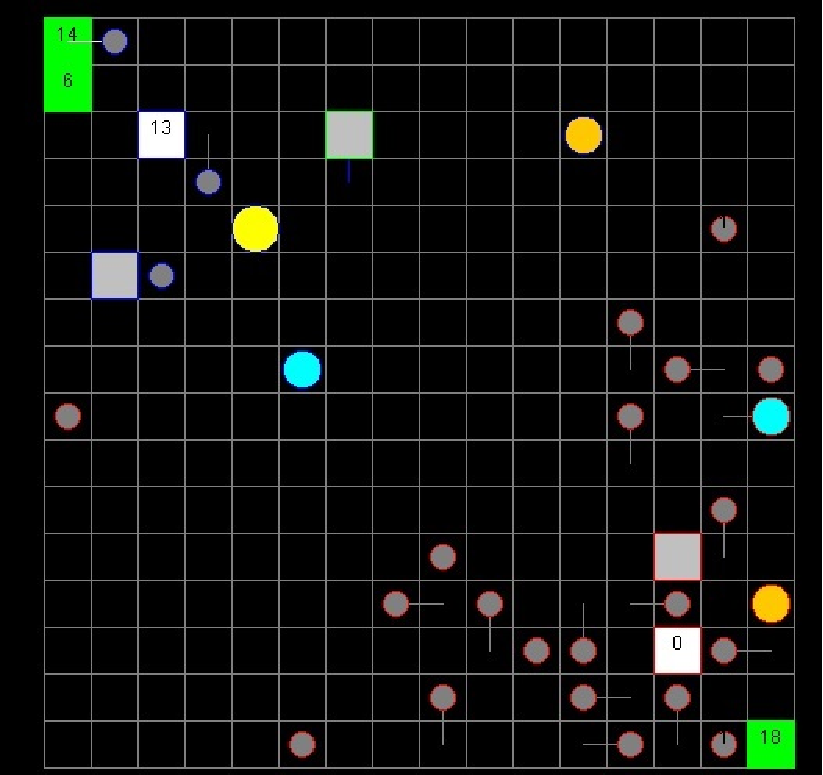
\includegraphics[width=0.5\textwidth]{fig/microrts.pdf}
 	\caption{Um exemplo de tela do MicroRTS}
 	\label{fig:microrts}
 \end{figure} 
 
 No ambiente há algumas estrategias implementadas, cada estrategia possui variações dos algoritmos. Algumas das estrategias são:
 \begin{itemize}
 	\item Minimax Alpha-Beta Search Strategies - O que muda entre as técnicas é o jeito com que é feito a expansão do grafo.
 	\item Monte Carlo Search Strategies - Executa jogadas aleatórias para planejar e após utiliza uma heurística para determinar em qual caminho seguir.
 \end{itemize}
 
 A plataforma já foi utilizada para aplicar técnica de IA. Por esse motivo a utilização desta plataforma se torna viável. A comparação entre as estrategias já existentes com a que estou propondo pode mostrar que a abordagem resulta em um melhor desempenho. 
 
 
 
 